% !TeX root = ../../../main.tex
\begin{figure}[htbp]
\begin{ChFiveFloatBody}

  \centering
  \begin{minipage}[t]{0.45\linewidth}\centering
    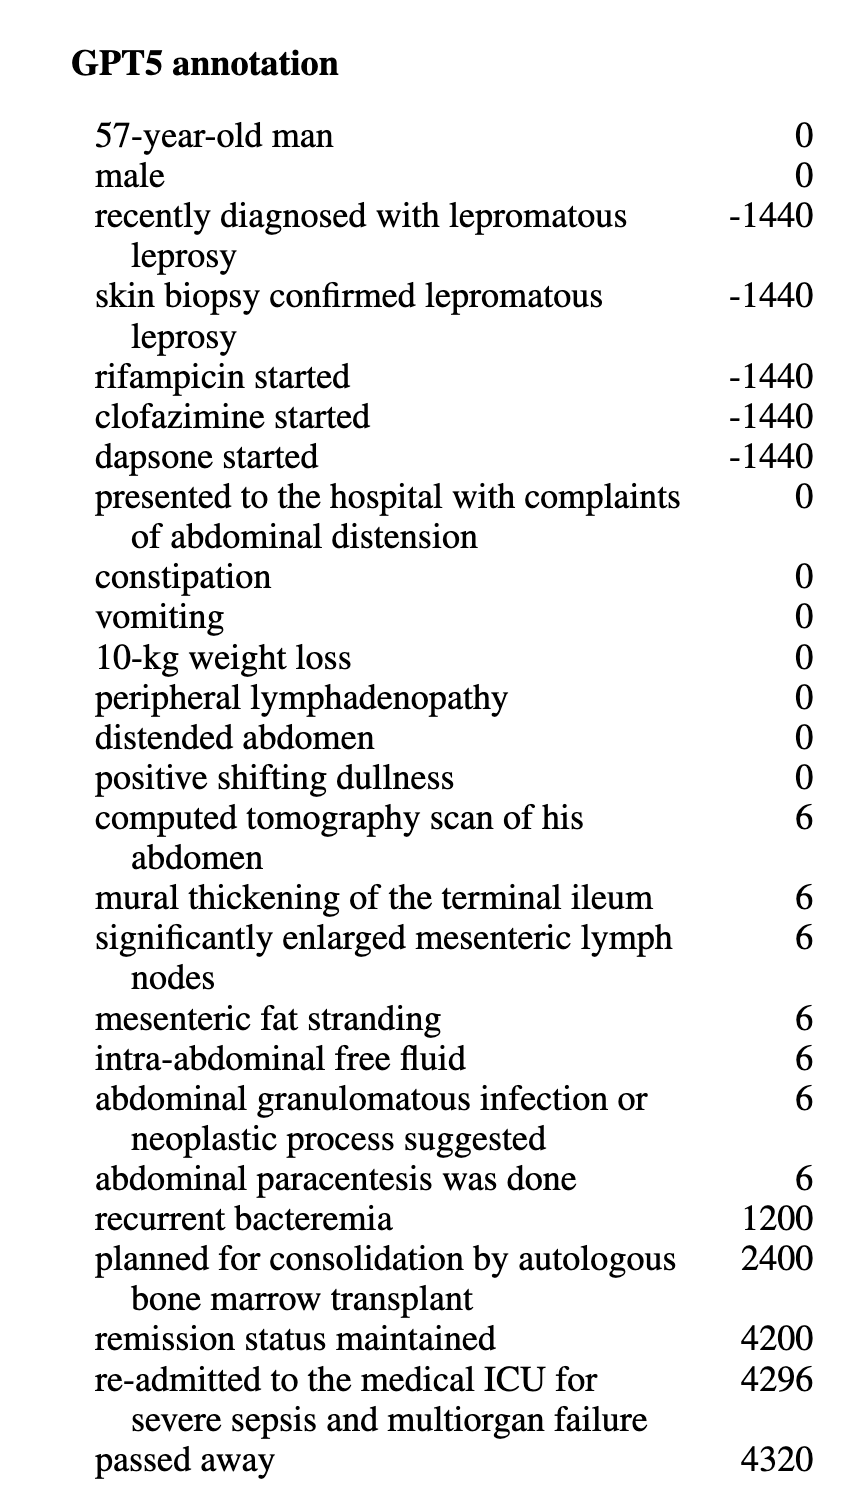
\includegraphics[width=0.9\linewidth]{Appendices/appendix-ch05/images/Scientific_data/Supplementary/example_TTS_for_paper/GPT5.png}
  \end{minipage}\hfill
  \begin{minipage}[t]{0.45\linewidth}\centering
    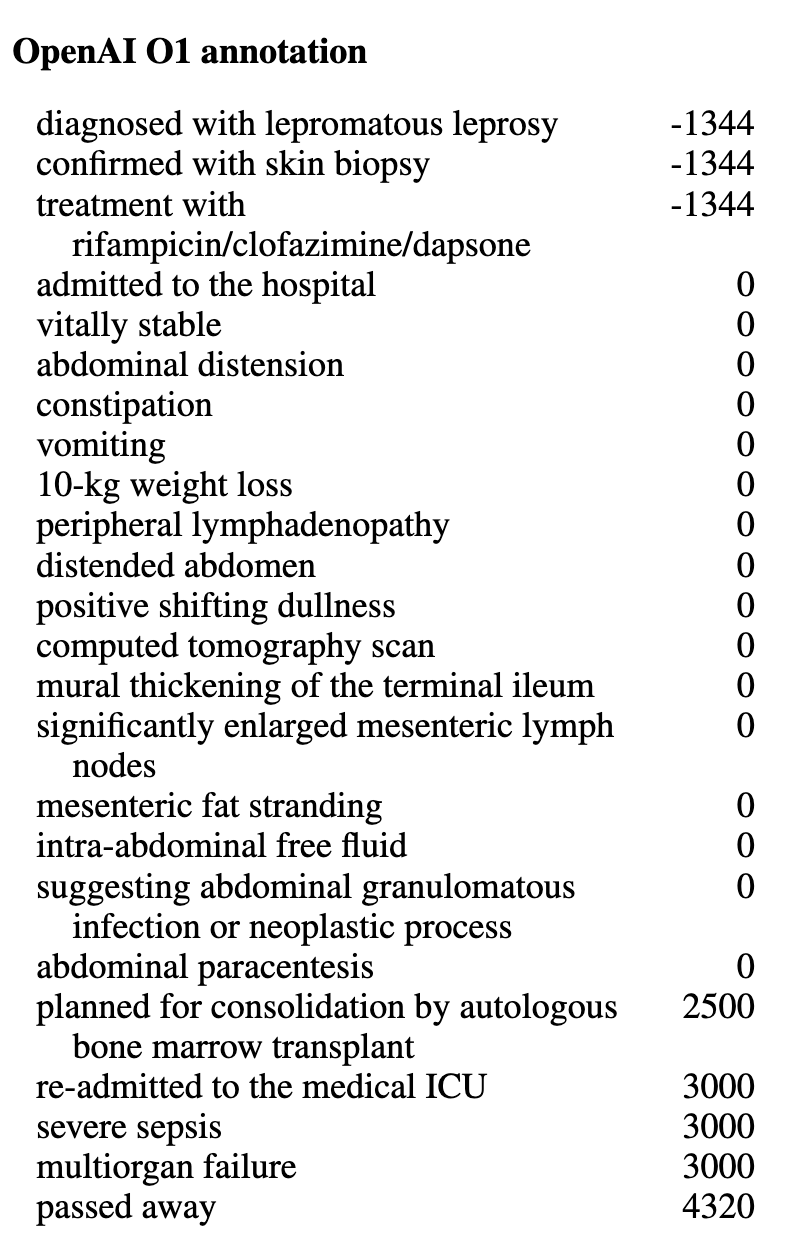
\includegraphics[width=0.9\linewidth]{Appendices/appendix-ch05/images/Scientific_data/Supplementary/example_TTS_for_paper/O1.png}
  \end{minipage}

  

  \begin{minipage}[t]{0.45\linewidth}\centering
    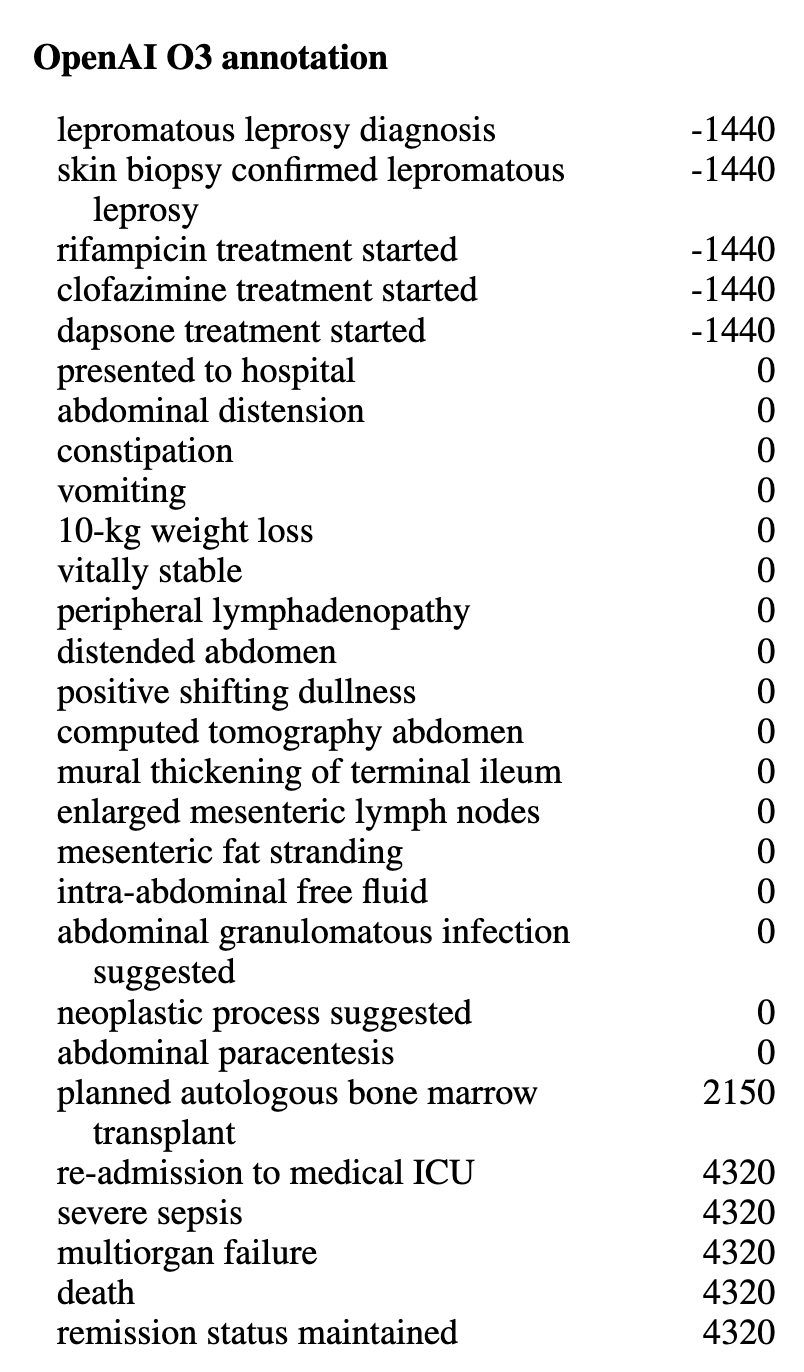
\includegraphics[width=0.9\linewidth]{Appendices/appendix-ch05/images/Scientific_data/Supplementary/example_TTS_for_paper/O3.png}
  \end{minipage}\hfill
  \begin{minipage}[t]{0.45\linewidth}\centering
    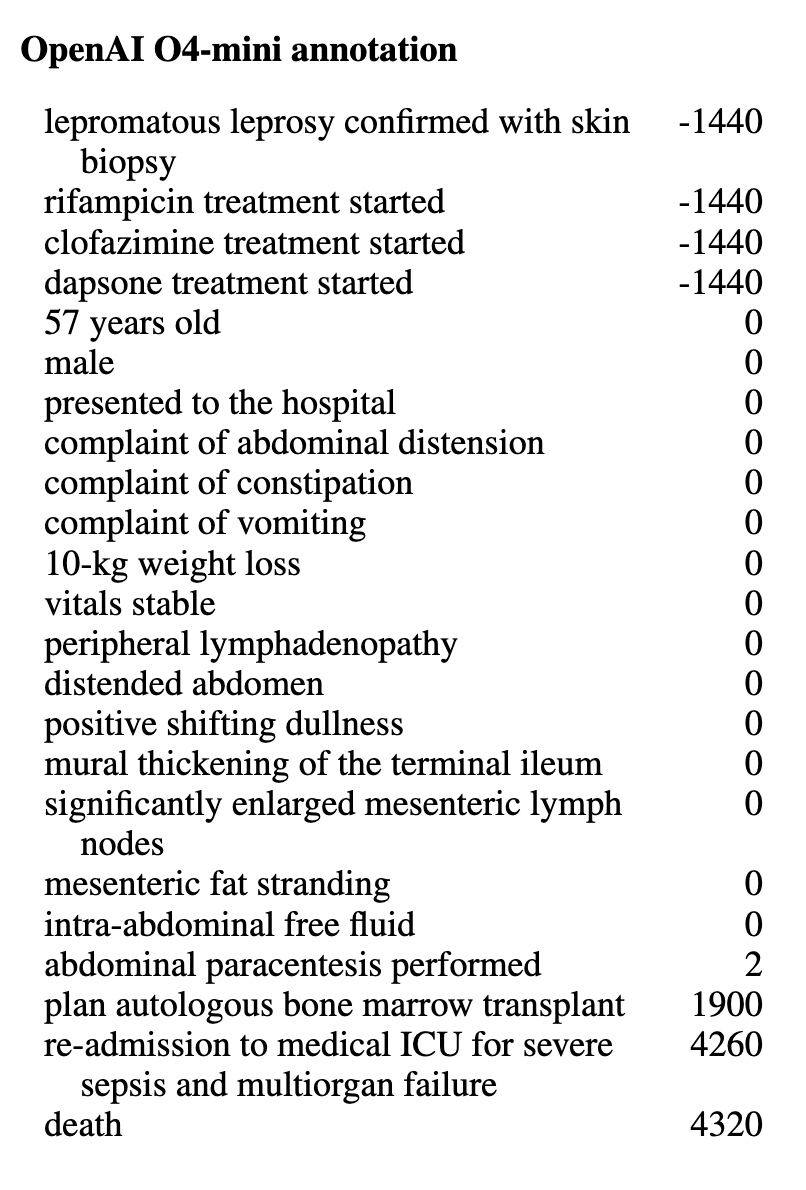
\includegraphics[width=0.9\linewidth]{Appendices/appendix-ch05/images/Scientific_data/Supplementary/example_TTS_for_paper/O4mini.png}
  \end{minipage}


  
  

\end{ChFiveFloatBody}
\caption{Comparison of temporal annotations generated by several LLMs for a representative case report (PMC10629858). The figure contrasts manual annotations with model-generated event–time
sequences, highlighting differences in event granularity, phrasing, duplicate event generation, and temporal normalization (e.g., variation in converting narrative expressions such as ``two
months before admission’’ into hour offsets). Long-range timestamp assignments (e.g., for transplant planning, ICU readmission, and death) show the greatest variability across models, whereas the overall ordering of major clinical events is largely preserved. This example illustrates characteristic
differences in how LLMs interpret, segment, and temporally anchor clinical narratives.}\ChFiveFloatLabel{ch05:fig:compare_llm_annotations}
\end{figure}